\problemname{Minequake}

The fully autonomous microbreweries installed in the abandoned Dwarven mines of Moravia are truly a testament to the ingenuinity and craftsmanship of Dwarvish engineering!
Alas, infrequent earthquakes rattle the mines, leading to misaligned funnels that spill precious liquid on the floor.
As the Exalted Lord of Brewery Safety it is your responsibility to turn off the machines in every hall in case of an earthquake.

Since walking through tunnels takes time, 
you will be late in turning of many of the machines.
You want to minimise the amount of spilled liquid.

\medskip
The Dwarven mines consist of $n$ halls connected by $n-1$ tunnels.
The entire system is connected, so it is possible to get from any hall to any of the others.
It takes one unit of time to traverse a tunnel.
Switching off a machines and traversing a hall takes no time.
In each hall, turning off the machines $t$~time after the earthquake spills $t$~liters of liquid.
You may not switch off any machines before the actual earthquake.
You can start in any of the halls.

\subsection*{Example}

In sample input~$1$, the mines look like this:

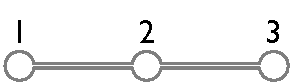
\includegraphics[width=.15\textwidth]{img/sample-1.pdf}

If you start in hall~$2$ and visit the rest of the halls in the order $2$, $1$, $2$, $3$, you can switch off their machines at time~$0$ (in hall $2$), time~$1$ (in hall $1$), and time~$3$ (in hall $3$).
This wastes $0+1+3=4$~liters.
If instead you start in hall~$1$ and visit the halls in the order $1$, $2$, $3$, the total penaly is $0+1+2=3$, which is better.

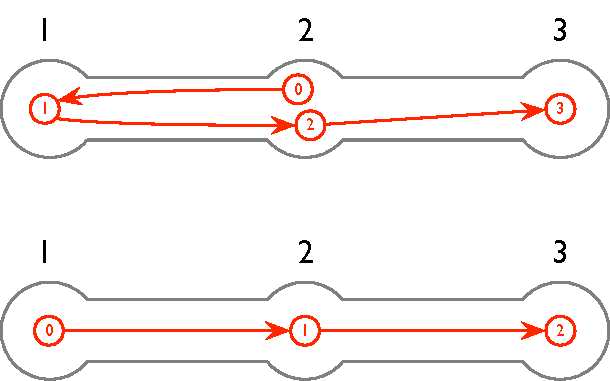
\includegraphics[width=.35\textwidth]{img/sample-1-ans.pdf}

\subsection*{Input}

The first line of input consists of the integer $n$, the number of halls.
We assume that $1\leq n\leq 100\,000$ and that the halls are numbered $1$, $\ldots$, $n$.
The next $n-1$ lines each contain two space-separated integers $u$ and $v$ with $1\leq u < v \leq n$, meaning that there is a tunnel between hall~$u$ and hall~$v$.

\subsection*{Output}

Print a single integer: the minimum amount of spilled liquid.

\subsection*{Constraints}

Your solution will be tested on a set of test groups, each worth a number of points.
Each test group contains a set of test cases.
To get the points for a test group you need to solve all test cases in the test group.
Your final score will be the maximum score of a single submission.

\medskip
\begin{tabular}{lll}
Group & Points & Constraints \\\hline
1 & 18 & no hall is incident to more than two tunnels\\
2 & 19 & at most one hall is incident to more than two tunnels\\
3 & 20 & $n\leq 10$\\
4 & 21 & $n\leq 1\,000$\\
5 & 22 & \emph{no additional constraints}
\end{tabular}
